\chapter{Images in Python}

An image is usually represented as three dimensional array of 8-bit
integers. numpy arrays are the most commonly used library for this
sort of data structure.

If you have an RGB image that is 480 pixels tall and 640 pixels wide,
you will need a $480 \times 640 \times 3$ numpy array.

There is a separate library (imageio) that:
\begin{itemize}
\item Reads an image file (like JPEG files) and creates a numpy array.
\item Writes a numpy array to a file in standard image formats
\end{itemize}

Let's create a simply python program that creates a file containing
all-black image that is 640 pixels wide and 480 pixels tall. Create a
file called \filename{create\_image.py}:

\begin{Verbatim}
import numpy as np
import imageio
import sys

# Check command-line arguments
if len(sys.argv) < 2:
    print(f"Usage {sys.argv[0]} <outfile>")
    sys.exit(1)

# Constants
IMAGE_WIDTH = 640
IMAGE_HEIGHT = 480

# Create an array of zeros
image = np.zeros((IMAGE_HEIGHT, IMAGE_WIDTH, 3), dtype=np.uint8)

# Write the array to the file
imageio.imwrite(sys.argv[1], image)
\end{Verbatim}

To run this, you will need to supply the name of the file you are
trying to create. The extension (like .png or .jpeg) will tell imageio
what format you want written. Run it now:

\begin{Verbatim}
python3 create_image.py blackness.png
\end{Verbatim}

Open the image to confirm that it is 640 pixels wide, 480 pixels tall, and completely black.

\section{Adding color}

Now, let's walk through through the image, pixel-by-pixel, adding some
red. We will gradually increase the red from 0 on the left to 255 on
the right.

\begin{Verbatim}[commandchars=\\\{\}]
import numpy as np
import imageio
import sys

# Check command-line arguments
if len(sys.argv) < 2:
    print(f"Usage {sys.argv[0]} <outfile>")
    sys.exit(1)

# Constants
IMAGE_WIDTH = 640
IMAGE_HEIGHT = 480

# Create an array of zeros
image = np.zeros((IMAGE_HEIGHT, IMAGE_WIDTH, 3), dtype=np.uint8)

\textbf{for col in range(IMAGE_WIDTH):}

    \textbf{# Red goes from 0 to 255 (left to right)}
    \textbf{r = int(col * 255.0 / IMAGE_WIDTH)}

    \textbf{# Update all the pixels in that column}
    \textbf{for row in range(IMAGE_HEIGHT):}
        \textbf{# Set the red pixel}
        \textbf{image[row, col, 0] = r}

# Write the array to the file
imageio.imwrite(sys.argv[1], image)
\end{Verbatim}

When you run the function to create a new image, it will be a fade
from black to red as you move from left to right:


\includegraphics[width=0.4\linewidth]{red.png}

Now, inside the inner loop, update the blue channel so that it goes
from zero at the top to 255 at the bottom:

\begin{Verbatim}[commandchars=\\\{\}]
    # Update all the pixels in that column
    for row in range(IMAGE_HEIGHT):

        # Update the red channel
        image[row,col,0] = r
        
        \textbf{# Blue goes from 0 to 255 (top to bottom)}
        \textbf{b = int(row * 255.0 / IMAGE_HEIGHT)}
        \textbf{image[row,col,2] = b}

imageio.imwrite(sys.argv[1], image)
\end{Verbatim}

When you run the program again, you will see the color fades from
black to blue as you go down the left side. As you go down the right
side, the color fades from red to magenta.

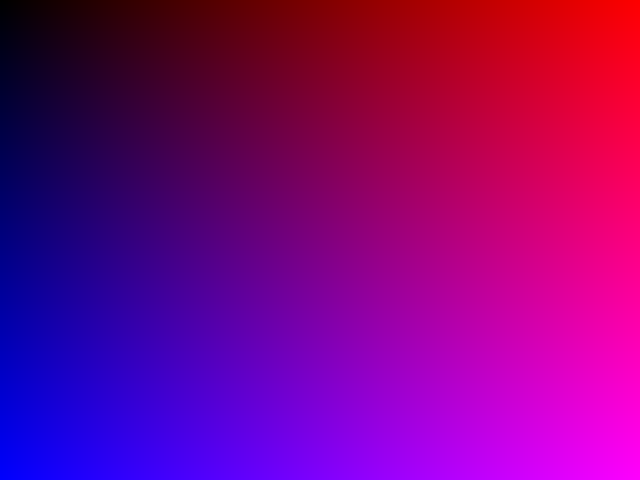
\includegraphics[width=0.4\linewidth]{rb.png}

Notice that red and blue with no green looks magenta to your eye.

Now lets add some stripes of green:

\begin{Verbatim}[commandchars=\\\{\}]
import numpy as np
import imageio
import sys

# Check command line arguments
if len(sys.argv) < 2:
    print(f"Usage {sys.argv[0]} <outfile>")
    sys.exit(1)

# Constants
IMAGE_WIDTH = 640
IMAGE_HEIGHT = 480
\textbf{STRIPE_WIDTH = 40}
\textbf{pattern_width = STRIPE_WIDTH * 2}

# Create an image of all zeros
image = np.zeros((IMAGE_HEIGHT, IMAGE_WIDTH, 3), dtype=np.uint8)

# Step from left to right
for col in range(IMAGE_WIDTH):

    # Red goes from 0 to 255 (left to right)
    r = int(col * 255.0 / IMAGE_WIDTH)

    \textbf{# Should I add green to this column?}
    \textbf{should_green = col % pattern_width > STRIPE_WIDTH}

    # Update all the pixels in that column
    for row in range(IMAGE_HEIGHT):

        # Update the red channel
        image[row,col,0] = r

        \textbf{# Should I add green to this pixel?}
        \textbf{if should_green:}
            \textbf{image[row,col,1] = 255}

        # Blue goes from 0 to 255 (top to bottom)
        b = int(row * 255.0 / IMAGE_HEIGHT)
        image[row,col,2] = b

imageio.imwrite(sys.argv[1], image)
\end{Verbatim}

When you run this version, you will see the previous image in half the
stripes.  In the other half, you will see that green fades to cyan
down the left side and yellow fades to white down the right side.

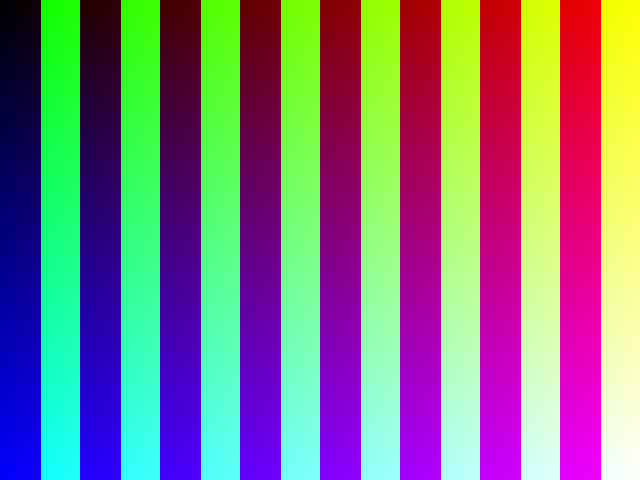
\includegraphics[width=0.4\linewidth]{rgb.png}

\section{Using an existing image}

imageio can also be used to read in any common image file
format. Let's read in an image and save each of the red, green, and blue
channels out as its own image.

Create a new file called \filename{separate\_image.py}:

\begin{Verbatim}
import imageio
import sys
import os

# Check command line arguments
if len(sys.argv) < 2:
    print(f"Usage {sys.argv[0]} <infile>")
    sys.exit(1)

# Read the image
path = sys.argv[1]
image = imageio.imread(path)

# What is the filename?
filename = os.path.basename(path)

# What is the shape of the array?
original_shape = image.shape

# Log it
print(f"Shape of {filename}:{original_shape}")

# Names of the colors for the filenames
colors = ['red','green','blue']

# Step through each of the colors
for i in range(3):

    # Create a new image
    newimage = np.zeros(original_shape, dtype=np.uint8)

    # Copy one channel
    newimage[:,:,i] = image[:,:,i]

    # Save to a file
    new_filename = f"{colors[i]}_{filename}"
    print(f"Writing {new_filename}")
    imageio.imwrite(new_filename, newimage)
\end{Verbatim}

Now you can run the program with any common RGB image type:

\begin{Verbatim}
python3 separate_image.py dog.jpg
\end{Verbatim}

This will create three images: \filename{red\_dog.jpg},
\filename{green\_dog.jpg}, and \filename{blue\_dog.jpg}.
